\documentclass[xcolor=dvipsnames]{beamer}

% ==== 主題 ====
\usetheme{metropolis}
\usefonttheme{professionalfonts}          % 不覆蓋你自訂的字型

% ==== 字型 ====
\usepackage{fontspec}
\usepackage{xeCJK}
\renewcommand{\familydefault}{\rmdefault} % 使用 serif 字體（重點）
\usefonttheme{professionalfonts}

% 西文字型：Times New Roman 的開源替代品
\setmainfont{TeX Gyre Termes}[
  Ligatures=TeX,
  BoldFont={* Bold},
  ItalicFont={* Italic}
]

% 中文字型（可改為思源宋體、標楷體等）
\setCJKmainfont{Noto Serif CJK TC}
\setCJKsansfont{Noto Sans CJK TC} % 有需要再用
\setCJKmonofont{Noto Sans Mono CJK TC}

% ==== 數學字型（與正文字體一致）====
\usepackage{unicode-math}
\setmathfont{TeX Gyre Termes Math}

% ==== 套件 ====
\usepackage{amsmath, amssymb}
\usepackage{graphicx}
\usepackage{hyperref}
\usepackage{minted}
\usepackage{fvextra}
\usepackage{xcolor}
\usepackage{booktabs}

% ==== 顏色設定（可選）====
\definecolor{MyBlue}{RGB}{3, 55, 105}
\setbeamercolor{structure}{fg=MyBlue}
\setbeamercolor{block title}{bg=MyBlue,fg=white}
\setbeamercolor{block body}{bg=blue!5}
\setbeamertemplate{section in toc}{%
  \inserttocsectionnumber.~\inserttocsection\par
}

\setminted{
    linenos,                % 行號
    frame=lines,            % 上下框線
    framesep=5pt,           % 程式碼與邊框距離
    numbersep=8pt,          % 行號與程式碼距離
    fontsize=\scriptsize,   % 字體大小
    breaklines,             % 自動換行
    tabsize=4,              % tab 寬度
    rulecolor=\color{black},% 框線顏色
    xleftmargin=1.5em       % 左側縮排
}

\title{Course Introduction \& Review 1}
\author{Tai, Wei Hsuan}
\date{week 1}

\begin{document}
	\begin{frame}
		\titlepage
	\end{frame}

    \begin{frame}
        \frametitle{Outline}
        \tableofcontents
    \end{frame}

    \section{課程介紹}

    \begin{frame}
        \frametitle{\href{https://drive.google.com/drive/folders/14Tkn-rddw0k1obeOxkWi00S43M0e9wlW?usp=sharing}{課程簡報}}
        \begin{figure}
            \centering
            
\includegraphics[width=0.7\textwidth]{src/qrcode.png}
        \end{figure}
    \end{frame}

    \begin{frame}
        \frametitle{進度安排}
        Zerojudge ID: bu3hTa
        \makebox[\linewidth][c]{%
            \begin{tabular}{cl cl}
            \toprule
            日期 & 主題 & 日期 & 主題 \\
            \midrule
            3/6  & 課程簡介、複習1   & 5/8 & STL簡介、stack, queue, deque \\
            3/20  & 複習2、時間複雜度簡介 & 5/15  & 單調隊列演算法 \\
            3/27 & 進階字串處理 & 5/22 & vector \\
            4/10 & 排序       & 5/29 & set, map, priority\_queue \\
            4/17  & 二分搜尋法    & 6/5 & STL的應用問題 \\
                &     & 6/12   & 期末考 \\
            \bottomrule
            \end{tabular}
        }
    \end{frame}

    \begin{frame}
        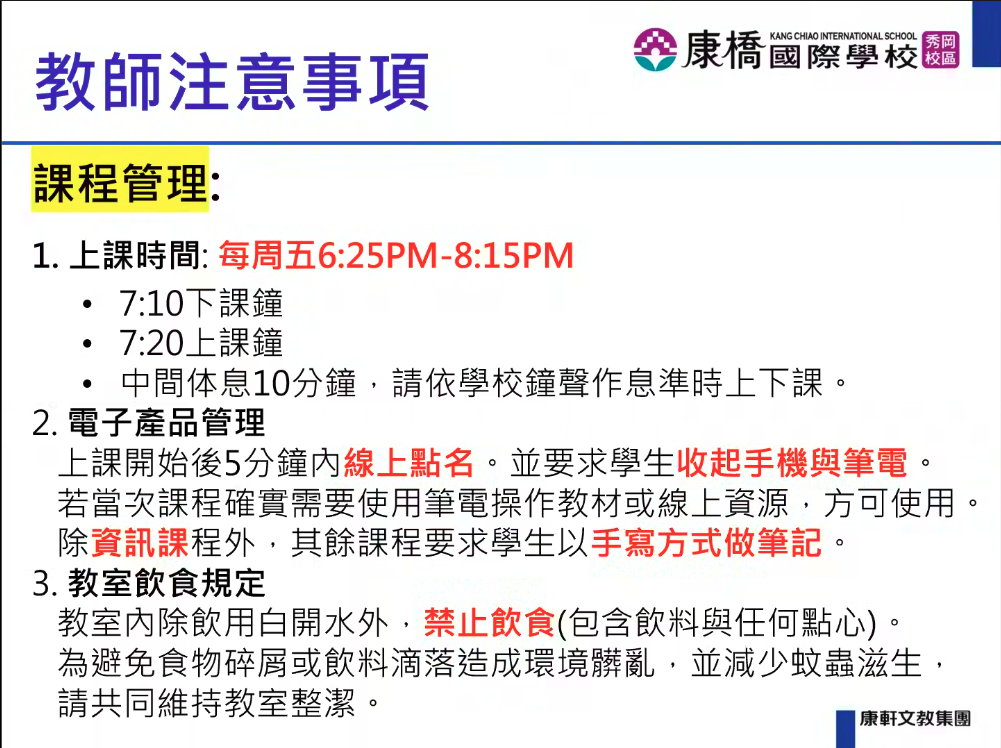
\includegraphics[width=\textwidth]{src/rule1.png}
    \end{frame}
    \begin{frame}
        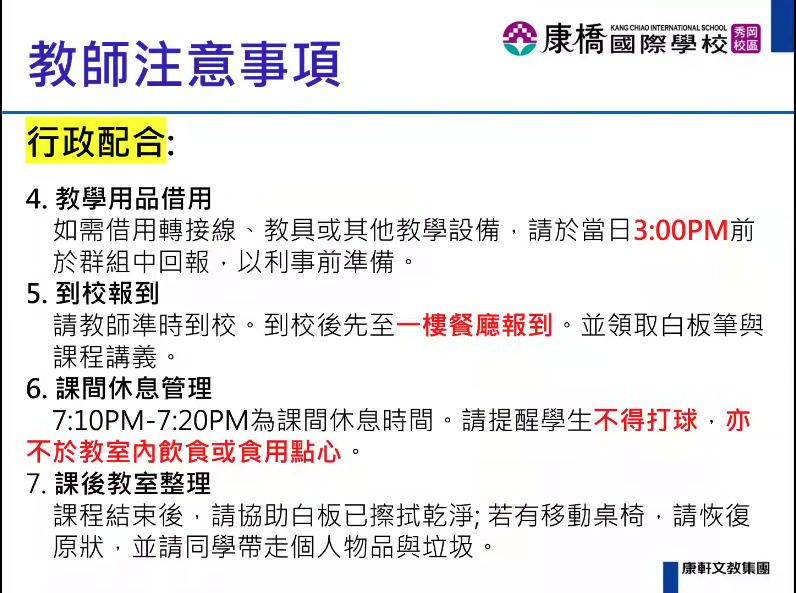
\includegraphics[width=\textwidth]{src/rule2.png}
    \end{frame}
    \section{Basic Structure of C++ Program}

    \begin{frame}[fragile]
        \frametitle{\href{https://zh.wikipedia.org/zh-tw/Hello_Worldtext}{Hello World!}}
        \begin{minted}{cpp}
        #include <iostream>
        using namespace std;

        int main() {
            cout << "Hello World!" << '\n';
            return 0;
        }
        \end{minted}
    \end{frame}

    \begin{frame}
        \frametitle{Three Main Parts}
        \begin{itemize}
            \item Header Files
            \item Namespaces
            \item Main Function
        \end{itemize}
    \end{frame}

    \begin{frame}[fragile]
        \frametitle{Basic Structure}
        \begin{minted}{cpp}
        #include <iostream> // Header Files
        using namespace std; // Namespaces
        int main() { // Main Function
            // do whatever you want
            return 0;
        }
        \end{minted}
    \end{frame}

    \begin{frame}[fragile]
        \frametitle{Basic Output}
        \begin{minted}{cpp}
        cout<<"[string]"<<[variable]<<'\n';
        \end{minted}
    \end{frame}

    \begin{frame}[fragile]
        \frametitle{Variables and Input}
        \begin{minted}{cpp}
        int a;
        cin >>a;
        \end{minted}
    \end{frame}

    \begin{frame}[fragile]
        \frametitle{Selection Structure}
        \begin{minted}{cpp}
        if(condition 1){
            // do something
        }else if(condition 2){
            // do something else
        }else{
            // do the rest
        }
        \end{minted}
    \end{frame}

    \begin{frame}[fragile]
        \frametitle{Loop Structure}
        \begin{minted}{cpp}
        for(int i=0;i<n;i++){
            // do something n times
        }

        while(condition){
            // do something while condition is true
        }
        \end{minted}
    \end{frame}

    \section{Problem Practice}
    \begin{frame}
        \frametitle{Practice 1: Output}
        \begin{columns}
            \column{0.5\textwidth}
            \begin{block}{Input}
            No input
            \end{block}
            \begin{block}{Output}
            Hello World!\;\textbackslash(\;\^\;o\;\^\;)/
            \end{block}
            \column{0.5\textwidth}
            \begin{block}{Sample Input}
            \end{block}
            \begin{block}{Sample Output}
            Hello World!\;\textbackslash(\;\^\;o\;\^\;)/
            \end{block}
        \end{columns}
    \end{frame}
    \begin{frame}
        \frametitle{Practice 2: Input and Output}
        \begin{columns}
            \column{0.5\textwidth}
            \begin{block}{Input}
            A name(string without spaces)
            \end{block}
            \begin{block}{Output}
            Hello, [name]! 
            \end{block}
            \column{0.5\textwidth}
            \begin{block}{Sample Input}
            Josh
            \end{block}
            \begin{block}{Sample Output}
            Hello, Josh! 
            \end{block}
        \end{columns}
    \end{frame}
    \begin{frame}
        \frametitle{Practice 3: Variables Practice}
        \begin{columns}
            \column{0.5\textwidth}
            \begin{block}{Input}
            Two numbers $a$ and $b$ (integers)
            \end{block}
            \begin{block}{Output}
            $a^b$
            \end{block}
            \column{0.5\textwidth}
            \begin{block}{Sample Input}
            2 3
            \end{block}
            \begin{block}{Sample Output}
            8
            \end{block}
        \end{columns}
    \end{frame}
    \begin{frame}
        \frametitle{Practice 4: Loops Practice}
        \begin{columns}
            \column{0.5\textwidth}
            \begin{block}{Input}
            A integer $n$
            \end{block}
            \begin{block}{Output}
            $n^{th}$ Fibonacci number (0-indexed, $F_0=0$, $F_1=1$)
            \end{block}
            \column{0.5\textwidth}
            \begin{block}{Sample Input}
            6
            \end{block}
            \begin{block}{Sample Output}
            8
            \end{block}
        \end{columns}
    \end{frame}

    \section{Zerojudge Practice}
    \begin{frame}
        \frametitle{Problem List}
        \begin{itemize}
            \item q001
            \item q027
            \item q089
            \item s137
            \item r168
            \item q916
        \end{itemize}
    \end{frame}


\end{document}